\documentclass[a4paper, 8pt]{article}
\usepackage[utf8x]{inputenc}
\usepackage{graphicx}
\usepackage{geometry}
\usepackage{amsmath}
\usepackage{mathenv}
\usepackage{amssymb}
\usepackage{amsfonts}
\usepackage{mathrsfs}
\usepackage{textcomp}
\geometry{hmargin = 2cm, vmargin = 1.5cm}

% OPENING
\title{SY 09 - P14 \\TP 3: Théorie de la décision}
\author{Ricard Tatiana, Mehr Jean-Christophe}
\date{}
\begin{document}

\maketitle

\textbf{ OBJECTIF DU TP} \\
\\* L’objectif de ce TP est de mettre en pratique deux théories de la décision qui sont le classifieur euclidien d’une part duquel nous allons tenter d’estimer son efficacité, et d’autre part la règle de Bayes en étudiant un problème de reconnaissance de cible.\\

\section*{Exercice 1 : Classifieur euclidien}
Le but de cet exercice est d’étudier les performances du classificateur euclidien sur des échantillons issus des deux classes $\omega_{1}$ et $\omega_{2}$ de $\mathbb{R}^{2}$ dont les distributions sont normales et de paramètres ($\mu_{1}$, $\Sigma_{1}$) et ($\mu_{2}$, $\Sigma_{2}$).

\subsection*{1) Simulation d'un échantillon}
En utilisant la fonction \textbf{mvrnorm} de la bibliothèque \textbf{MASS}, nous avons écrit la fonction \textbf{simul} qui nous retourne
un échantillon de taille \textit{n} tiré suivant une proportion $\pi$ d'exemples issus de la classe $\omega_{1}$.
Pour chaque exemple, nous avons, dans un premier temps, tiré au hasard la classe dont il est issu,
avant de le générer en utilisant les paramètres adéquats.\\
Voilà les résultats obtenus graphiquement :
Nous avons utilisé pour cette fonction les cinq situations suivantes :\\
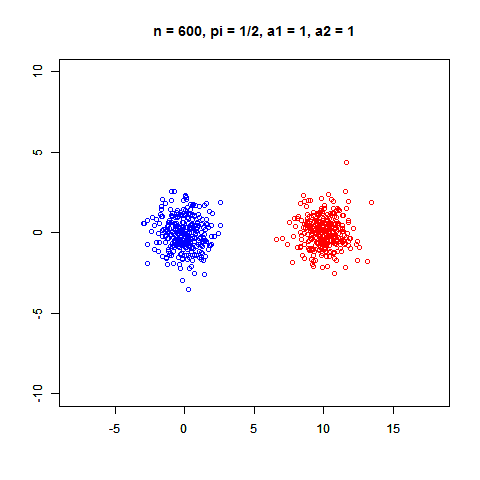
\includegraphics[height = 7cm, width = 7cm]{plots/plot_simul_1.png}
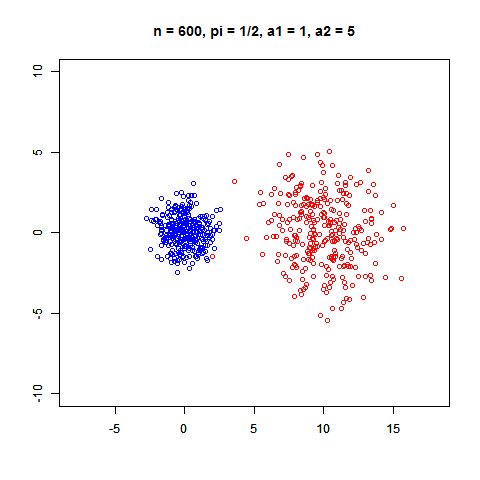
\includegraphics[height = 7cm, width = 7cm]{plots/plot_simul_2.png}\\
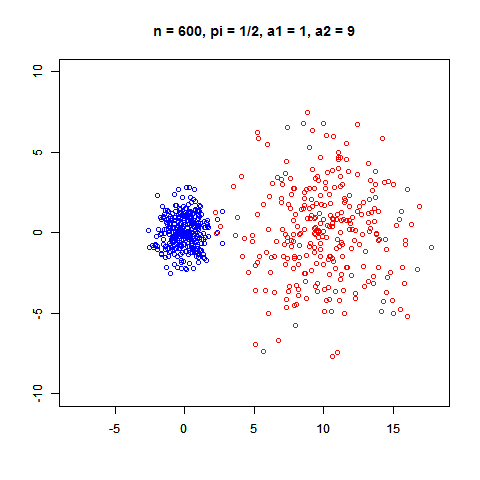
\includegraphics[height = 7cm, width = 7cm]{plots/plot_simul_3.png}
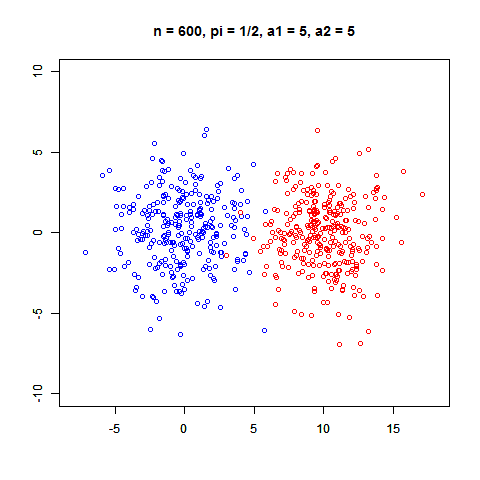
\includegraphics[height = 7cm, width = 7cm]{plots/plot_simul_4.png}\\
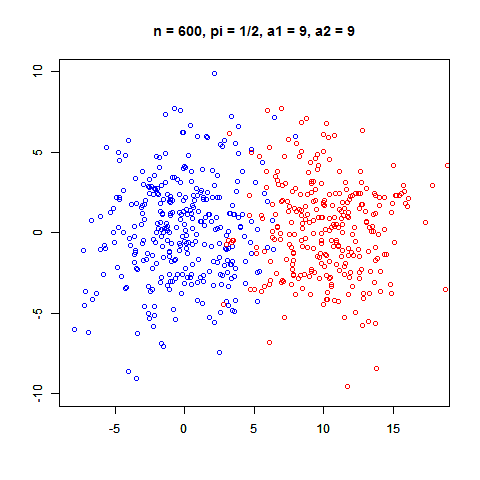
\includegraphics[height = 7cm, width = 7cm]{plots/plot_simul_5.png}\\
Grâce à ces simulations, nous observons que plus la variance est élevée plus la dispersion des point est grande (autour de la moyenne), ils sont moins concentrés.
 Il apparaît qu’à partir d’une certaine valeur de variance (exemple de la cinquième figure) il existe un chevauchement entre les classes $\omega_{1}$ et $\omega_{2}$.\\
Il devient alors plus difficile de les distinguer et on peut d’ores et déjà supposer que la probabilité d’erreur sera plus importante.\\ \\
\newpage
\noindent
\subsection*{2) Estimation de la probabilité d'erreur}
Désormais nous allons chercher à estimer la probabilité d’erreur associée au classifieur Euclidien. Pour cela nous avons séparé en deux parties de même cardinal nos échantillons initiaux contenant les classes $\omega_{1}$ et $\omega_{2}$.\\ La première partie est l’échantillon d’apprentissage permettant d’apprendre les moyennes $\mu_{1}$ et $\mu_{2}$. La seconde partie est l’ensemble de tests permettant d’estimer le taux d’erreur de classifieur Euclidien sur ces données.\\\\
Utiliser un ensemble de test nous permet d’estimer la performance du classifieur. Nous avons pour celà tout d’abord écris une fonction règle Euclidienne qui correspond au classifieur Euclidien. Cette fonction compare les distances entre d’une observation x et l’estimateur$\mu_{1}$ puis $\mu_{2}$ et renvoie alors la classe dont x est le plus proche. Ensuite nous avons réalisé une fonction erreurEstimee qui calcul le nombre d’erreur de classification que notre classifieur a commis sur l’ensemble de test divisé par le cardinal de cet ensemble. Cette fonction renvoie donc le pourcentage d’erreur estimé.\\
$\\ \\$
Le calcul de la probabilité d'erreur en fonction des estimations de moyennes $\mu_{1}$ et $\mu_{2}$ nous donne les valeurs suivantes :\\ \\
\begin{tabular}{|c|c|}
\hline
Variance & Probabilité d'erreur ($\%$) \\
\hline
($\Sigma_{1}$ = 1, $\Sigma_{2}$ = 1) & 0 \\
\hline
($\Sigma_{1}$ = 1, $\Sigma_{2}$ = 5) & 0.33 \\
\hline
($\Sigma_{1}$ = 1 ,$\Sigma_{2}$ = 9) & 2.67 \\
\hline
($\Sigma_{1}$ = 5, $\Sigma_{2}$ = 5) & 1.33 \\
\hline
($\Sigma_{1}$ = 9, $\Sigma_{2}$ = 9) & 5.67 \\
\hline
\end{tabular}
\\ \\
\\Les résultats ci-dessus nous montrent bien que plus la variance est élevée, plus le taux d’erreur augmente et donc moins le classifieur Euclidien est performant. Ceci s’explique par le fait que la règle Euclidienne évalue la distance euclidenne entre chacun des points et les centres des deux classes. Il attribue ensuite à ce point la classe dont le centre est le plus proche. \\\\
De ce fait, lorsque la dispersion d’une classe est grande, les échantillons ont tendance à se chevaucher. Ainsi certains points se retrouve mal classifiés car il peut se retrouver plus proche du centre de l’autre classe si c’est un point éloigné du centre de sa propre classe (grande dispersion), le taux d’erreur est alors plus élevé.\\ En ce qui concerne la simulation 4, où $\Sigma_{1}$ = 5 et $\Sigma_{2}$ = 5, nous remarquons que le taux d’erreur est moins élevé que la simulation 3 où $\Sigma_{1}$= 1 et $\Sigma_{2}$ = 9. \\
Cela laisse à penser qu’en terme d’efficacité il vaut mieux disposer de deux classes  de variances modérées que d’une classe de variance faible et une autre très élevée. En effet bien que les deux sommes des variances de chaque simulation soient égales (10) une variance très élevée rendra un taux d’erreur plus important car se rapprochera plus facilement du centre de la classe à variance réduite (il n’y aura qu’un seul type d’erreur).


\newpage
\subsection*{3) Probabilité d'erreur moyenne}
Nous cherchons maintenant à observer la  probabilité d’erreur moyenne, nous avons créé une fonction permettant de répéter les opérations précédentes 10 fois. À partir de ces dix simulations pour chacun des cas nous avons calculé la moyenne, la variance et un intervalle de confiance de niveau 5% sur l’espérance de la probabilité d’erreur. L’intervalle de confiance étant calculé grâce au test de Student.\\
$\\\\$
Cette fonction nous permet de récupérer les données suivantes :\\ \\
\begin{tabular}{|c|c|c|c|}
\hline
Variance & Moyenne du taux d'erreur & Variance du taux d'erreur (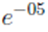
\includegraphics[height = 0.25cm, width = 0.25cm]{plots/e.png}) & Interface de confiance de niveau 5$\%$ \\
\hline
($\Sigma_{1}$ = 1, $\Sigma_{2}$ = 1) & 0$\%$ & 0 & [0;0]\\
\hline
($\Sigma_{1}$ = 1, $\Sigma_{2}$ = 5) & 0.57$\%$ & 2.481481 & [0.21$\%$;0.923$\%$] \\
\hline
($\Sigma_{1}$ = 1 ,$\Sigma_{2}$ = 9) & 2.03$\%$ & 1.481481 & [1.276$\%$;2.791$\%$] \\
\hline
($\Sigma_{1}$ = 5, $\Sigma_{2}$ = 5) & 1.3$\%$ & 3.567901 & [0.873$\%$;1.727$\%$] \\
\hline
($\Sigma_{1}$ = 9, $\Sigma_{2}$ = 9) & 4.6$\%$ & 2.04444 & [3.577$\%$;5.623$\%$] \\
\hline
\end{tabular}$\\\\\\$
Nous remarquons que répéter l’opération permet d’abaisser le pourcentage d’erreur et de rendre la classifieur euclidien plus efficace.

\newpage
\section*{Exercice 2 : Règle de Bayes}

\subsection*{1. Montrer que les distributions \textit{$f_{1}$} et \textit{$f_{2}$} sont des distributions normales.}
La fonction de densité d'une variable aléatoire suivant une loi normale est de la forme \textit{f}(\textit{x}) =
$\frac{1}{\sigma(2\pi)^{\frac{1}{2}}}$\textit{$e^{-\frac{1}{2}(\frac{x - \mu}{\sigma})^{2}}$}\\
Nous avons donc pour \textit{$f_{1}$}(x) :\\
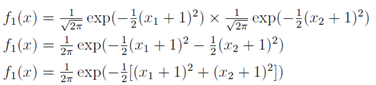
\includegraphics[height = 2cm, width = 8cm]{plots/f1.png}
\\
Nous savons qu'une loi normale \textit{f}(\textit{x}) bidimensionelle est de la forme :\\
\textit{f}(\textit{x}) = $\frac{1}{2\pi det(\Sigma)^{{2}}}$\textit{$e^-\frac{1}{2}(x - \mu)^{T} \Sigma^{-1}(x - \mu)$}\\
Par identification avec la formule vue précedemment nous trouvons donc $\Sigma_{1} =
\begin{pmatrix}
1 & 0 \\
0 & 1
\end{pmatrix}$
et $\mu_{1} =
\begin{pmatrix}
-1 \\
-1
\end{pmatrix}$
\\
De la meme facon, on trouve pour \textit{$f_{2}$}(x) :
$\Sigma_{2} =
\begin{pmatrix}
1 & 0 \\
0 & 1
\end{pmatrix}$
et $\mu_{2} =
\begin{pmatrix}
1 \\
1
\end{pmatrix}$
\\
\\
Les lois \textit{$f_{1}$} et \textit{$f_{2}$} suivent donc des lois normales bidimensionelles avec les paramètres vu ci dessus.

\newpage
\subsection*{2. Générer un échantillon de \textit{n} réalisations issues des deux classes $\omega_{1}$ et $\omega_{2}$.}

Pour générer un échantillon de \textit{n}n réalisations issues des deux classes $\omega_{1}$ et $\omega_{2}$ en proportions égales\\
($\pi_{1}$ = $\pi_{2}$ = 0.5), nous avons utilisé la fonction \textbf{simul} écrite précédemment.\\
Pour chacun des échantillons, nous avons ensuite déterminé les estimations des différents paramètres de \textit{$f_{1}$} et \textit{$f_{2}$}.\\
Pour les valeurs de \textit{n} suivantes : 10, 100, 1000, 10 000, 100 000, nous obtenons donc les résultats suivants :\\ \\
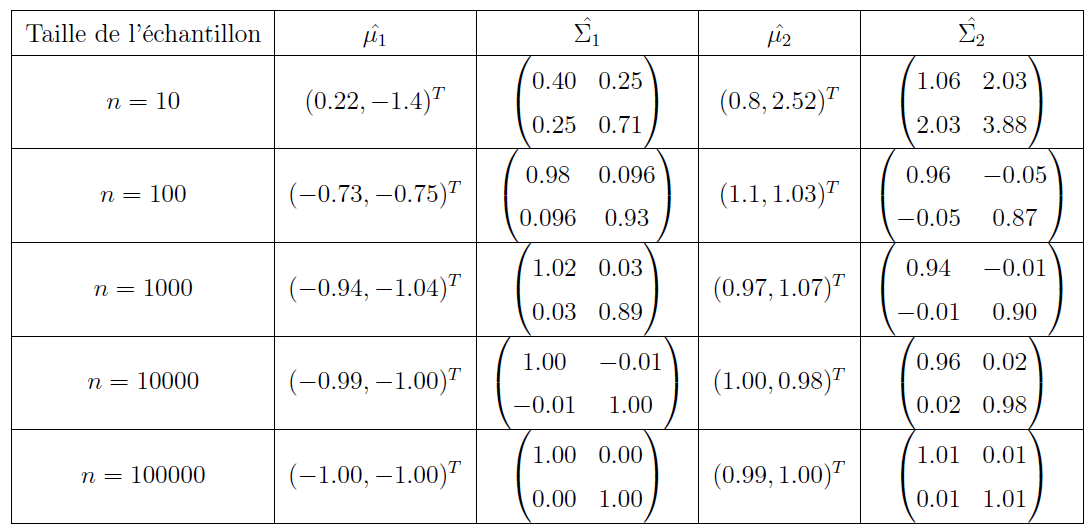
\includegraphics[height = 8cm, width = 15cm]{plots/f2.png}
\\ Nous avons pu observer que plus n était grand, plus on se rapprochait de la valeur théorique.\\ \\

\subsection*{3. Montrer que les courbes d'iso-densité sont des cercles.}

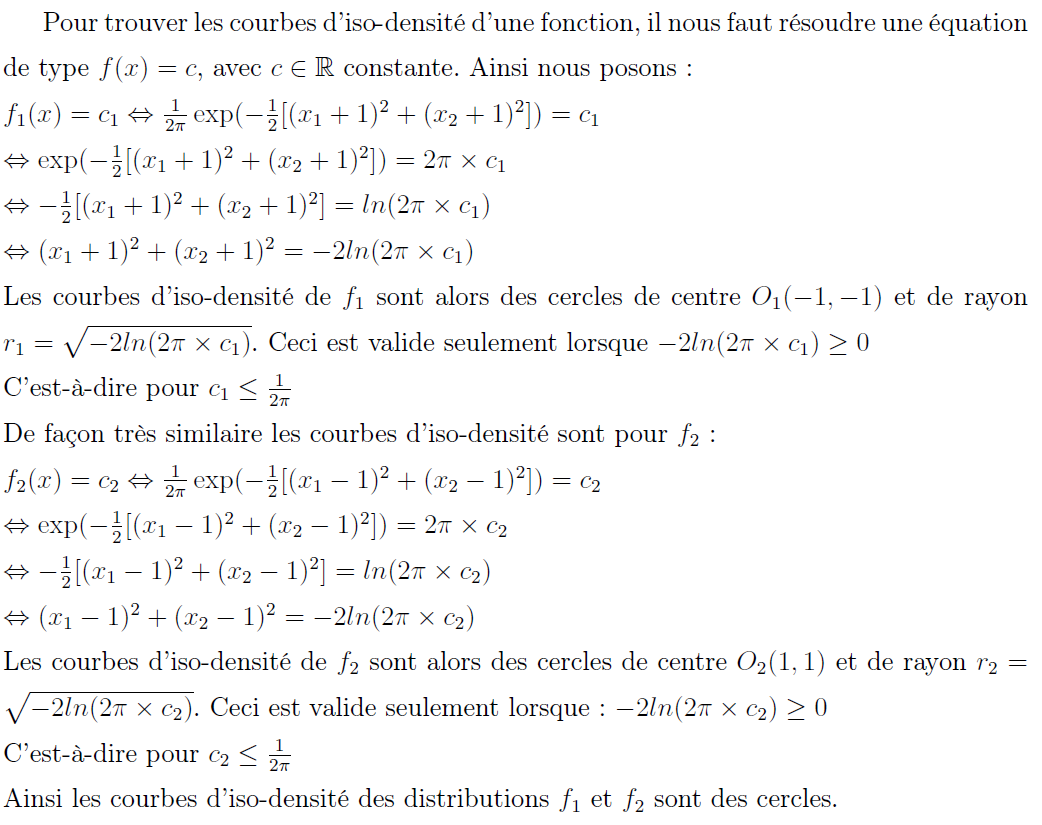
\includegraphics[height = 10cm, width = 13cm]{plots/f3.png}
\\
\newpage

\subsection*{4. Règle de Bayes.}

\subsubsection*{(a) Donner l'expression de la règle de Bayes $\delta^{*}$ pour ce problème.}

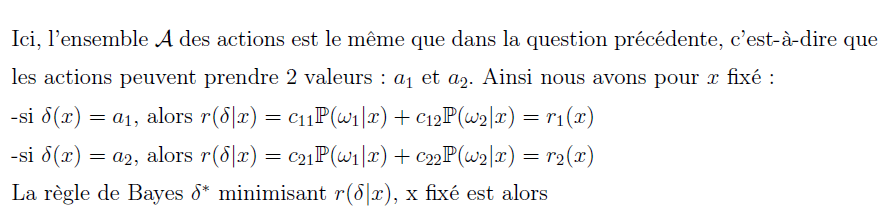
\includegraphics[height = 3cm, width = 13cm]{plots/f4.png}\\
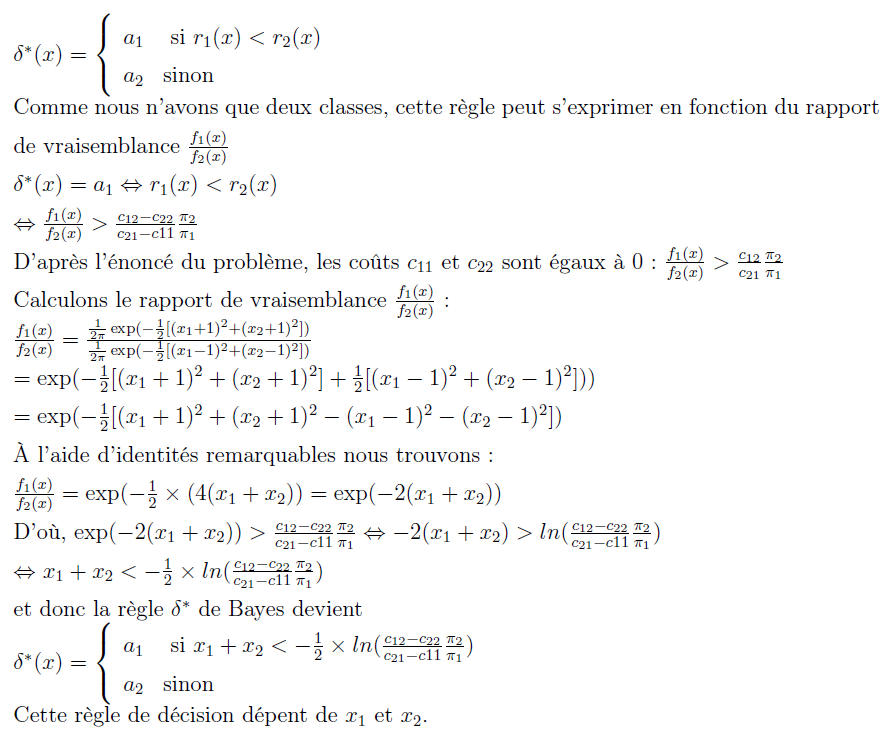
\includegraphics[height = 12cm, width = 13cm]{plots/f5.png}

\subsubsection*{(b et c) Tracer les frontières de décision correspondantes dans le plan (\textit{$X_{1}$}, \textit{$X_{2}$}) et donner une estimation des risques $\alpha$ et $\beta$.}
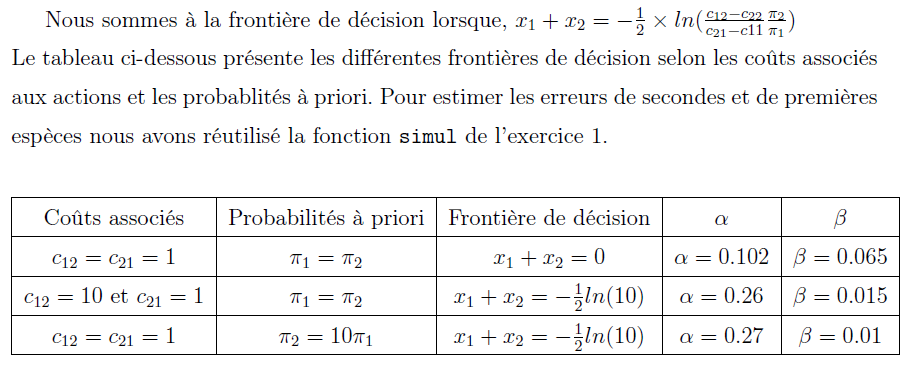
\includegraphics[height = 6cm, width = 14cm]{plots/f6.png}\\
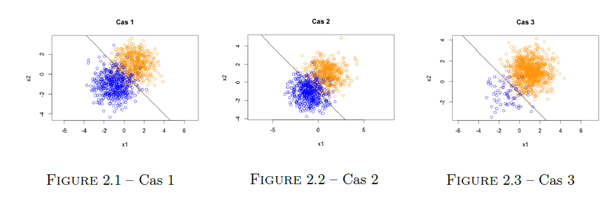
\includegraphics[height = 6cm, width = 12cm]{plots/plot_simul_6.png}\\ \\

Nous remarquons que pour la cas 1, la frontière se situe quasiment au milieu. On peut l'expliquer par le afit que le coût d'une erreur d'affectation à une classe et les probabilités sont identiques.\\
Le risque de classer les points dans $\omega_{1}$ et $\omega_{2}$  est donc identique.\\
Pour le cas 2, les coûts sont différents : en effet, c12 est 10 fois plus important que c21 et les probabibilés semblent toujours égales. Ainsi, il est dix fois plus coûteux de mal classer un individu appartenant à la classe $\omega_{2}$. Sur le graphique, la règle de Baynes place la frontière plus près d'$\omega_{1}$. La règle de Bayes classifie donc mal une grande quantité d'éléments de cette classe afin d'être sûr de ne pas mal classifier d'éléments coûteux (corroboré par les valeurs d'$\alpha$ et $\beta$ avec $\alpha$ très grand).\\ \\
Pour finir, dans le cas 3 les coûts sont une nouvelle fois les memes, cependant les proportions sont différentes.\\
La proportion des individus dans $\omega_{2}$ est quasiment dix fois plus grande que celle d'$\omega_{1}$. Pour équilibrer les risques, la règle de Bayes place donc la frontière plus proche d'$\omega_{1}$. Ceci explique donc pourquoi l'erreur de second type $\beta$  soit faible et que le risque $alpha$ soit beaucoup plus grand !


\newpage
\section*{Conclusion}
Nous avons finalement pu dans ce TP étudier un classifieur euclidien et les effets des valeurs des variances sur le pourcentage d’erreur.
En outre nous avons pu observer que comme dans beaucoup de cas, répéter l’expérience permettait de réduire ce pourcentage d’erreur.\\
Dans le deuxième exercice nous avons pu étudier la règle de Bayes et observer l’influence de la proportion des classes et des coûts sur les frontières de décisions, la rêgles de Bayes tentant de minimiser le pourcentage d’erreur et le coût  global.\\
Les règles de décisions permettent donc de classifier des éléments en fonction d’observations et de paramètres prédéfini, il est alors possible de jouer sur ces paramètres et sur la taille de l’échantillon afin d’influencer ces décisions.


\end{document}
